\documentclass{article}
\usepackage[utf8]{inputenc}
\usepackage{geometry, parskip, hyperref}
\usepackage{amsfonts, amsmath}
\usepackage{pgfplots, graphicx}
\usepackage{caption, subcaption}


\title{
    \textbf{ECE250: Signals \& Systems} \\
    \large{Assignment 1: Report}
}

\author{\href{mailto:divyajeet21529@iiitd.ac.in}{Divyajeet Singh (2021529)}}

\date{September 15, 2022}

\geometry{a4paper, left=25mm, right=25mm, top=25mm, bottom=25mm}
\pgfplotsset{compat=1.18}

\begin{document}
    \maketitle

    \textbf{Assumptions:}

    \begin{enumerate}
        \item The signal $u[n]$ is the unit-step signal, defined below: \begin{equation}
            u[n] = \begin{cases}
                1 & \text{ if } n \geq 0 \\
                0 & \text{ if } n < 0
            \end{cases}
        \end{equation}

        \item $p[q[n]]$ means scaling the signal $q[n]$ by $p$, when $p \in \mathbb{R}$.
    \end{enumerate}

    \textbf{Question: 5}

    \begin{enumerate}

        \item $x[n] = n[u[n] - u[n-10]] + 10e^{-0.3(n-10)}[u[n-10] - u[n-20]],\ 0 \leq n \leq 20$
        \begin{figure}[h]
            \centering
            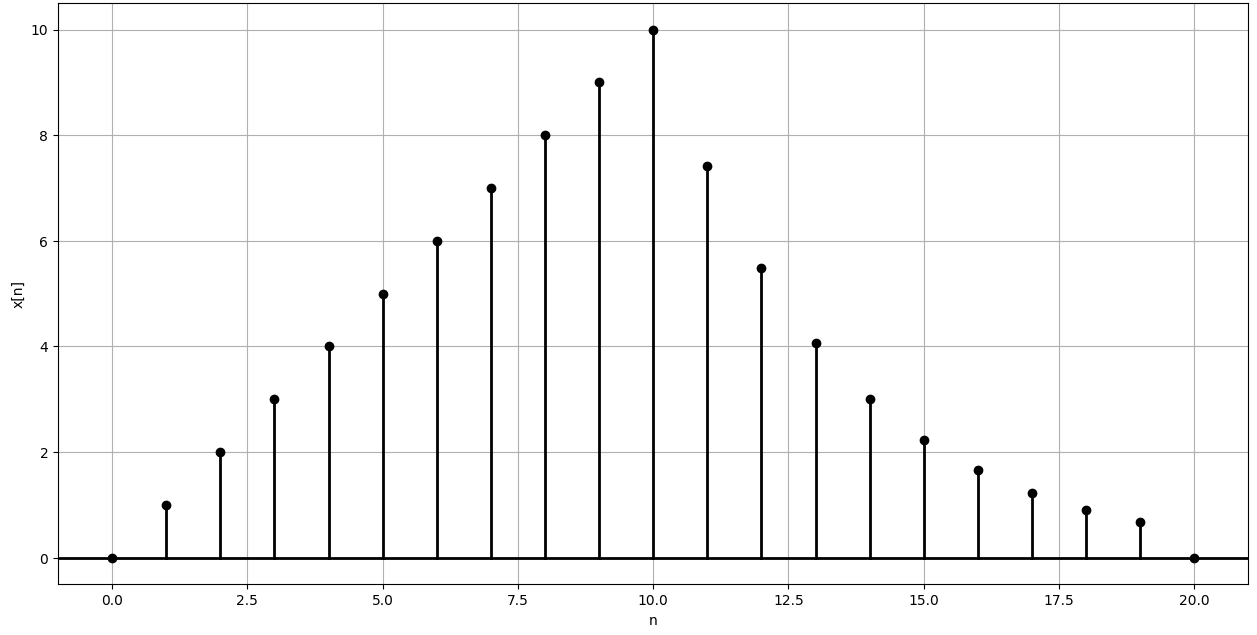
\includegraphics[scale=0.39]{./Assets/solution-5-i.png}
        \end{figure}

        \item $y[n] = \cos{[0.03 \pi n]} + u[n],\ 0 \leq n \leq 50$
        \begin{figure}[h]
            \centering
            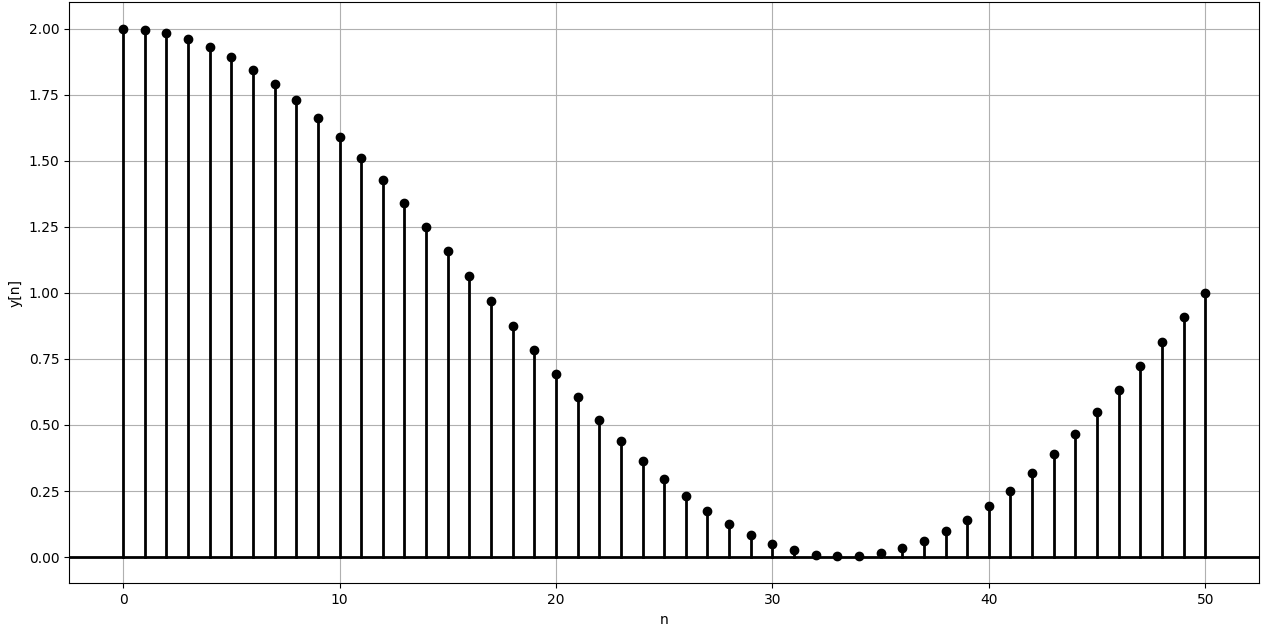
\includegraphics[scale=0.39]{./Assets/solution-5-ii.png}
        \end{figure}

    \end{enumerate}

    \textbf{Question: 6}

    Given signal: $z[n] = u[n] - u[n-10]$

    \begin{align}
        \text{Even}\{z[n]\} &= \frac{z[n] + z[-n]}{2} \\
        \text{Odd}\{z[n]\} &= \frac{z[n] - z[-n]}{2}
    \end{align}

    \begin{figure}[h]
        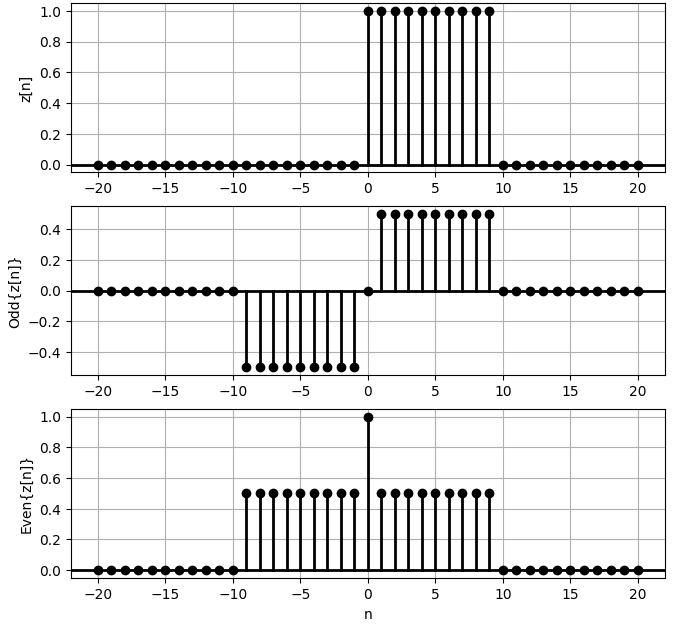
\includegraphics[scale=0.9]{./Assets/solution-6.png}
        \caption*{Subplots for \textbf{Question: 6}}
    \end{figure}

    Some inferences:
    \begin{enumerate}
        \item The even part of $z[n]$ is symmetric about the $x$-axis, $y = 0$.
        \item The odd part of $z[n]$ is symmetric about the line $y = x$.
        \item It is also (visually) clear that $z[n] = \text{Odd}\{x[n]\} + \text{Even}\{x[n]\}$.
    \end{enumerate}
\end{document}